
\section{Algoritmi}
\label{cap:algorithms}

\subsection{Prim con Binary Heap}

La versione vista a lezione di Prim vista in aula prevede i seguenti step:

\begin{enumerate}
    \item Creare una lista $\pi$ non inizializzata di dimensione pari a quella dei vertici del grafo;
    \item Per ogni vertice, inizializzare le chiavi a $+\infty$;
    \item Assegnare il valore $0$ ad una chiave arbitraria (radice dell'MST);
    \item Creare una coda di priorità basata su Min Heap che contenga tutti i nodi non ancora inseriti nell'MST;
    \item Fino a che la coda non è vuota, estrarre il nodo $u$ avente chiave minore dalla coda;
    \item Iterare lungo i vertici $v$ adiacenti al nodo $u$ dentro al ciclo $while$;
    \item Se $v$ appartiene alla coda e il peso dell'arco $(u, v)$ è $<$ della chiave di $v$, inserire l'arco $(u, v)$ allo Spanning Tree $\pi$ e decrementare il valore della chiave di $v$ al peso dell'arco $(u, v)$;
    \item Restituire $\pi$.
\end{enumerate}

\noindent Il listato \ref{listing:prim-binary-heap} contiene la nostra implementazione dell'algoritmo, step per step. La coda di priorità usata si basa su una struttura dati di tipo Min Binary Heap. \\

\begin{listing}[!ht]
\begin{minted}{c++}
// PrimBinaryHeap/prim_binary_heap_mst.h

// step 1
auto vertexes = adj_map_graph.get_vertexes();
const size_t n_stop = vertexes.size();
std::vector<Edge<Label, Weight>> mst(n_stop);

// step 2
constexpr Weight Infinity = std::numeric_limits<Weight>::max();
std::vector<Weight> keys(vertexes.size(), Infinity);

// step 3
keys.at(0) = Weight(0);

// step 4
constexpr bool IsAlreadyHeap = true;
auto min_pq(priority_queue::make_min_priority_queue<IsAlreadyHeap>(
    std::move(keys), std::move(vertexes)));

while (!(min_pq.empty() && n_stop == mst.size())) {
  // step 5
  auto u = min_pq.top();
  min_pq.pop();

  // step 6
  for (const auto [v, weight] : adj_map_graph.adjacent_vertexes(u)) {
    // step 7
    if (min_pq.contains(v) && weight < min_pq.key_at(v)) {
      min_pq.update_key(weight, v);
      mst.at(v) = Edge<Label, Weight>(u, v, weight);
    }
  }
}

// step 8
return mst;
\end{minted}
\caption{Implementazione di PrimBinaryHeap. I commenti del file originale sono stati omessi per una maggiore compattezza.}
\label{listing:prim-binary-heap}
\end{listing}

\subsubsection{Osservazioni}

\begin{itemize}
    \item Abbiamo utilizzato \mintinline{c++}{std::numeric_limits<Weight>::max()} per inizializzare le chiavi al valore massimo assumibile dal tipo generico \mintinline{c++}{Weight}, che è istanziato come \mintinline{c++}{long}. Il massimo valore rappresentabile è quindi \mintinline{c++}{2147483647L}. \\

    \item Poiché scegliamo sempre il primo nodo per inizializzare a 0 la chiave dello step 3, il container \textit{keys} rispetta già la proprietà di Min Heap. La coda di priorità è quindi creata in tempo \complexityConstant{}. \\

    \item Se l'MST che stiamo costruendo arriva a contenere $n - 1$ archi prima che la coda sia svuotata, usciamo prematuramente dal ciclo. \\

    \item Determinare se la coda contiene un nodo $v$ e se il peso $weight$ corrente è minore della chiave associata a $v$ ha complessità temporale \complexityConstant{} ammortizzata.\\

    \item Aggiornare il valore della chiave associata ad un nodo $v$ ha complessità temporale pari a \complexityLogN{}.\\
\end{itemize}


\subsection{Kruskal Simple}

La versione vista a lezione di Kruskal vista in aula prevede i seguenti step:

\begin{enumerate}
    \item Inizializzare l'oggetto da restituire in output $A$ (che conterrà quindi l'MST) come insieme vuoto;
    \item Ordinare gli archi del grafo per costo non decrescente;
    \item Iterare lungo gli archi in tale ordine;
    \item Aggiungere $edge$ ad $A$, ma solo se $A \cup \{ edge \}$ è aciclico;
    \item Restituire $A$.
\end{enumerate}

\noindent Il listato \ref{listing:kruskal-simple} contiene la nostra implementazione dell'algoritmo, step per step.

\begin{listing}[!ht]
\begin{minted}{c++}
// KruskalNaive/kruskal_naive_mst.h

// step 1
const size_t n = adj_map_graph.vertexes_size();
AdjacencyMapGraph<Label, Weight> mst_set_graph({}, n);

// step 2
auto edges = adj_map_graph.get_sorted_edges(std::less<>{});

DFSCycleDetection<Label, Weight> dfs(&mst_set_graph);

// step 3
for (auto it = edges.cbegin();
     !(it == edges.cend() && n == mst_set_graph.vertexes_size()); ++it) {
  const auto &edge = *it;

  // step 4
  mst_set_graph.add_edge(edge);
  if (dfs.has_cycle()) {
    mst_set_graph.remove_edge(edge);
  }
}

// step 5
return mst_set_graph.get_edges();
\end{minted}
\caption{Implementazione di KruskalNaive. I commenti del file originale sono stati omessi per una maggiore compattezza.}
\label{listing:kruskal-simple}
\end{listing}

\noindent L'algoritmo Kruskal Naive è stato implementato a partire dallo pseudo codice visto in classe. A partire da questo ci si è subito accorti che una delle peculiarità di tale algoritmo e la necessità di verificare ad ogni inserimento di un arco di peso minimo la presenza di un ciclo nell'MST calcolato. Per ottenere tale funzionalità abbiamo deciso di modificare DFS in maniera da rilevare la presenza di un ciclo in un grafo. Per fare questo è stato creata la classe DFSCycleDetection, che è possibile ritrovare nella cartella ``Shared'', che data la rappresentazione del grafo e richiamando l'apposito metodo \codeinline{has\_cycle()} è in grado di rilevare la presenza di un ciclo all'interno di esso usando per l'appunto una visita in profondità.\\

\noindent Abbiamo pertanto dovuto modificare DFS nel seguente modo:
\begin{itemize}
	\item non è necessario avere una label per ogni arco che etichetti quell'arco come ``DISCOVERY EDGE'' o ``BACK EDGE''
	\item quando un arco verrebbe etichettato come ``BACK EDGE'' nello pseudo codice visto in classe possiamo affermare che nel grafo è presente un ciclo. Non è necessario riscostruire tutto il ciclo come visto in un ulteriore modifica di DFS in classe.
	\item al posto di tener traccia di ogni arco se è stato visitato o meno attraverso l'attributo ID visto in clase, è stato deciso di creare un set di archi già visitati dove l'inseriemento e la ricerca avviene in tempo costante.
	\item per essere sicuri di non prendere in considerazione il vertice da cui viene lanciata ricorsivamente la DFS (ossia per non lanciare DFS sul nodo padre) è stata passata alla ricorsione il vertice padre, in modo che quando si scansiona la lista di adiacenza del vertice in considerazione non si consideri il vertice padre, simulando così il comportamento della funzione \codeinline{opposite(v,e)} nello pseudo codice.
\end{itemize}

\noindent Per risolvere il problema di più di un eventuale componenente connessa nel grafo, vengono sempre scansionati tutti i nodi non ancora visitati attraverso un ciclo \codeinline{for} su tutti i vertici del grafo, come visto in classe.

\subsubsection{Osservazioni}

\begin{itemize}
    \item Abbiamo utilizzato \mintinline{c++}{adj_map_graph.get_sorted_edges(std::less<>{})} per ricevere un \mintinline{c++}{std::vector<Edge<Label, Weight>>} contenente gli archi in ordine non decrescente. Questa operazione costa tempo \complexityMLogM{} e usa il comparatore generico \mintinline{c++}{std::less<>}.\\

    \item Nello pseudo-codice non viene esplicitato in modo concreto come effettuare la verifica della ciclicità, i.e. verificare se $A \cup \{ e \}$ sia aciclico, lasciando così campo libero all'implementazione. Tra i vari modi di verificare la ciclicità abbiamo scelto di adattare l'algoritmo Depth-First Search per questo scopo.\\

    \item Se l'MST che stiamo costruendo arriva a contenere $n$ vertici prima di aver attraversato tutti gli archi, usciamo prematuramente dal ciclo.\\

    \item Il modo più ``comodo'' che abbiamo a disposizione per verificare se $A \cup \{ e \}$ abbia un ciclo, dove la $A$ dell'algoritmo visto a lezione corrisponde all'oggetto $mst\_set\_graph$ e $e$ corrisponde alla variabile $edge$, è aggiungere $edge$ a $mst\_set\_graph$ ed eventualmente rimuoverlo subito dopo in caso $dfs$ abbia individuato la presenza di un ciclo.\\

    \item Menzioniamo anche la gestione dei self loop o altri casi particolari che possiamo ritrovare nei grafi in input. Per fare questo ci aiutiamo con questi 2 esempi di base, raffigurati in figura~\ref{fig:SelfLoop}.

\begin{figure}[h]
	\caption{Esempi particolari di grafi da gestire}
	\centering
	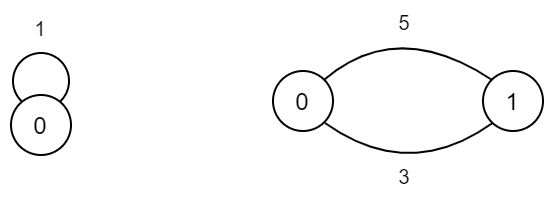
\includegraphics[width=0.7\textwidth]{./images/ExampleSelfLoop.png}
	\label{fig:SelfLoop}
\end{figure}

    Partendo dal caso di sinistra in cui esiste un nodo con un self loop, la funzione $has\_cycle\_$ $helper\_rec()$ è comunque in grado di rilevare la presenza di tale ciclo. Infatti come è possibile vedere dal listato \ref{listing:dfs-cycle} una volta lanciata la DFS sul nodo 0, la condizione dell'if sarà vera, in quanto il nodo 0 risulterà già visitato.

\begin{listing}[!ht]
\begin{minted}{c++}
// Shared/DFSCycleDetection.h

bool has_cycle_helper_rec(
    const Label &v, std::unordered_set<Label> &visited,
    const Label &parent = std::numeric_limits<Label>::max()) const {
  // segna il nodo corrente v come visitato
  visited.insert(v);

  // visita i nodi vicini del nodo corrente
  for (const auto &uw : adj_map_graph_ptr->adj_map.at(v)) {
    const auto &u = uw.first;

    // se il nodo corrente è diverso da suo padre, abbiamo 2 modi diversi
    // di segnalare la presenza di un ciclo:
    // 1) se il nodo u è già stato visitato, vi è un ciclo
    // 2) se l'invocazione ricorsiva con u come nodo sorgente ha ritornato
    // true, vi è un ciclo
    if (u != parent &&
        (visited.count(u) || has_cycle_helper_rec(u, visited, v))) {
      return true;
    }
  }

  return false;
}
\end{minted}
\caption{Funzione \codeinline{has\_cycle\_helper\_rec()} per la rilevazione di cicli}
\label{listing:dfs-cycle}
\end{listing}

    Per quanto riguarda invece l'esempio a destra in figura ~\ref{fig:SelfLoop}, viene automaticamente gestito dalle scelta implementativa fatta per la rappresentazione interna di un grafo. Infatti tale esempio, preso come input verrebbe trasformato in un grafo in cui sussiste un solo arco tra il nodo 0 e 1. L'arco che verrebbe preso in considerazione sarebbe quello di peso più basso, mentre l'altro viene scartato automaticamente. Pertanto all'interno della nostra struttura dati per rappresentare i grafi non sarà mai possibile avere nodi collegati in questo modo\\

    \item Un altra ulteriore ottimizzazione di tale algoritmo è la verifica ad ogni aggiunta di un nuovo arco che non crea un ciclo nel grafo, della soglia massima di archi che un MST può avere, che come visto in classe è pari al numero di nodi totali del grafo - 1. Pertanto non appena l'MST che si sta calcolando raggiunge la soglia prestabilità e possibile ritornare immediatamente l'MST.

\end{itemize}


\subsection{Kruskal con Disjoint Set}

La versione vista a lezione di Kruskal con Disjoint-Set (Union-Find) vista in aula prevede i seguenti step:

\begin{enumerate}
    \item Inizializzare l'oggetto da restituire in output $A$ (che conterrà quindi l'MST) come insieme vuoto;
    \item Inizializzare una struttura dati Disjoint-Set con la lista di vertici del grafo;
    \item Ordinare gli archi del grafo per costo non decrescente;
    \item Iterare lungo gli archi $e = (v, w)$ in tale ordine;
    \item Se $v$ e $w$ non sono connessi, aggiungere il loro arco ad $A$;
    \item Aggiornare la struttura dati Disjoint-Set unendo $v$ e $w$;
    \item Restituire $A$.
\end{enumerate}

\noindent Il listato \ref{listing:kruskal-union-find} contiene la nostra implementazione dell'algoritmo, step per step.

\begin{listing}[!ht]
\begin{minted}{c++}
// KruskalUnionFind/kruskal_mst.h

// step 1
std::vector<Edge<Label, Weight>> mst;
const size_t n_stop = adj_map_graph.vertexes_size() - 1;
mst.reserve(n_stop);

// step 2
auto vertexes = adj_map_graph.get_vertexes();
disjoint_set::DisjointSet<Label> disjoint_set(std::move(vertexes));

// step 3
const auto edges = adj_map_graph.get_sorted_edges(std::less<>{});

// step 4
for (auto it = edges.cbegin(); !(it == edges.cend() && n_stop == mst.size());
     ++it) {
  const auto &edge = *it;
  const auto &[v, w, _] = edge;

  if (!disjoint_set.are_connected(v, w)) {
    // step 5
    mst.push_back(edge);

    // step 6
    disjoint_set.unite(v, w);
  }
}

// step 7
return mst;
\end{minted}
\caption{Implementazione di KruskalUnionFind. I commenti del file originale sono stati omessi per una maggiore compattezza.}
\label{listing:kruskal-union-find}
\end{listing}

\subsubsection{Osservazioni}
\begin{itemize}
    \item Come osservato per KruskalNaive, abbiamo utilizzato il metodo  \mintinline{c++}{get_sorted_edges} \mintinline{c++}{(std::less<>{})} per ricevere un \mintinline{c++}{std::vector<Edge<Label, Weight>>} contenente gli archi in ordine non decrescente. \\

    \item Se l'MST che stiamo costruendo arriva a contenere $n - 1$ archi prima di aver attraversato tutti gli archi del grafo originale, usciamo prematuramente dal ciclo $for$. \\

\end{itemize}


% L'algoritmo di Kruskal con Disjoint Set implementato risulta essere in buona parte fedele a quello già visto in classe, con al differenze che è stato anche ottimizzata la condizione di terminazione, che prevede che al raggiungimento di n-1 archi all'interno dell'mst costruito, l'algoritmo termina restituendo l'mst calcolato fino a quel momento. Per implementare completamente questo algoritmo efficiente di Kruskal è necessario anche la creazione di un Disjoint Set: per fare ciò si e definita una classe astratta di base chiamata "DisjointSetBase" per poi implementarla con la classe "DisjointSet" e "DisjointCompressed" che non fanno altro che implementare i metodi astratti find e unite.
